\begin{WrapText}[t!]

\textbf{How can energy be ``free''?}

Energy is never actually free, but from the context of any thermodynamic system only some internal energy is free to cross the system barrier after entropy imposes its tax. In \our discussion, \we use free energy as a unifying metric across various domains. Consider the relationships between Gibbs free energy $G$, Helmholtz free energy $F$, Grand potential $\mathrm{\GFPPhi_{G}}$, and Kullback Leibler divergence $\kld{p}{q}$\citep[2]{Hafner2020}:

\begin{alignat*}{4}
&& G    &{} = {}&& H + PV && - TS \\
&& F    &{} = {}&& U      && - TS \\
&& \mathrm{\GFPPhi_{G}} &{} = {}&& E      && - TS - \mu N \\
&& \underbrace{ \kld{p}{q} }_{\text{free energy}} &{} = {}&& \stackengine{0pt}{\phantom{H + PV}}{\underbrace{ H(p,q) }_{\mathclap{\text{bound energy}}} }{U}{l}{F}{T}{L} && - \underbrace{ H(p) }_{\text{entropy}}
\end{alignat*}

% \[{{} \underbrace{\phantom{\kld{p}{q}}}_{\mathclap{\text{free energy}}}}  \underbrace{\phantom{H + PV}}_{ \mathclap {\text{bound energy} }} \phantom{- {}}\underbrace{ \phantom{ TS - \mu N } }_{\mathclap{\text{entropy}}} \phantom{\underbrace{}_{}}\]

%& \kld{p}{q} &&{} = {}&& H(p,q) && - H(p) \\[-2.7ex]
%& {\underbrace{\phantom{\kld{p}{q}}}_{\text{free energy}}} && && \underbrace{\phantom{H + PV}}_{\text{bound energy}} && \phantom{- {}}\underbrace{ \phantom{ TS - \mu N } }_{\text{entropy}} 

%& \underbrace{ \kld{p}{q} }_{\text{free energy}} &&{} = {}&& \stackengine{0pt}{\phantom{H + PV}}{\underbrace{ H(p,q) }_{\text{bound energy}}}{U}{c}{F}{T}{L}  && - \underbrace{ H(p) }_{\text{entropy}}

Also note interdisciplinary similarities in measures of difference:
\begin{itemize}
 \item energetic inequalities
 \item neuron firing and predictive coding
 \item (allostatic) stress
 \item economic disequilibrium
 \item the definition of a problem
\end{itemize}

\end{WrapText}

In all natural settings, free energy minimization is the norm, and its stagnation or increase is an exception: objects descend potential wells; virtual particles dissapate; the princple of least action obtains a minimal route for system evolution. In turn, decrease of free energy accompanies increase in entropy: structured arangements evaporate; gas pressures equalize; wavefunctions spread out. Notably, the Casmir force directly attracts of repels matter to maximize expected energy entropy in a way none of fundamental forces account for. (See Box ``How can energy be ``free''?'').

Neural networks represent a thermodynamic system of weights and activations, so it is only propper to extend the free energy minimizing motif in deep learning. Minimizing Kullback Leibler divergence between a model $p_\theta(y|x)$ on a data-generating distribution $\tau(x,y)$ has the convenient property of decreasing expected loss while also encouraging maximum entropy: $\min_\theta \kld{ p_\theta(y|x)\tau(x) }{ \tau(x,y) } = H(p_\theta(y|x)\tau(x), \tau(x,y)) - H(p_\theta(y|x)\tau(x))$ Additionally, the thermodynamic perspective identifies phase transitions in training which if properly understood can accelerate convergence.

Returning to our information efficency discussion from above, while we seek to maximize the information conductivity from the training data to the model, the objective during inference is reversed. Machine learning seeks to build models that react minimally to inputs noise. Even within a neural network, each layer may be understood as `absorbing' some of the data's energy as it travels to the output layer. With tools from linear algebra, it is easy to observe that each layer when interpretted as a random variable bijector can only output as much free energy as it recieves. Like a resistor chain, as activations ascend a classic DNN heirarchy, they may experience various coordinate transforms, but their expected information-energy--their entropy--only grows, hence minimizing free energy.

Life stands in defiance to the entropic trend, yet even in the struggle for survival, living systems continually optimize energy expendature. By the energy-information relationship, this means minimal information transfer and greatest potential for intelligence. For example, homeostatic mechanisms work to equalize energy production and consumption. This results in minimal free energy, optimal energy expendature, and ``survival intelligence'' (CITE). Genetic code likewise gives the muscular-skeletal system innate ``mechanical intelligence'' which `ofloads' some of the locomotive learning that a vertabrae's brain must perform. (Davide Zappetti CITE but that article is about robots not natural systems). From allostatic perspective, living systems represent a prior expectation of their environmental state and adapt their input and output modalities to the expected range of energy transfer. It follows that as actual and expected environments diverge, stress increases and survival imposes a greator information and energetic tax to maintain order. Again, probability expectation maximization accompanies energy minimization, hence control over the environment and intelligence.

It should be noted that intelligently meeting the energy challange in nature is not simply about on storing away as much energy as possible, but equalizing energy intake and expenderture. Sustained positive free energy is just debilitating as negative extremes.\footnote{In mobile life forms, selection pressures favor this extreme over the other. As this is not a common natural stressor, most animals simply do not need to carry the mechanisms to intelligently handle high amounts of free energy and suffer from resulting stress. } For instance, chronic elevated levels of mobilized energy and its indicators such as blood sugar, free fatty acids, cortisol, and blood pressure are associated with inflammation, diabetes, immunosuppression, ulceration, corinary heart disease, and hypertension. Likewise, extreme stressor exposure often maladaptively leads to PTSD. (GIVE SOME MORE MENTAL DISORDERS)

\begin{wrapfigure}{r}{0.5\textwidth}
 \centering
 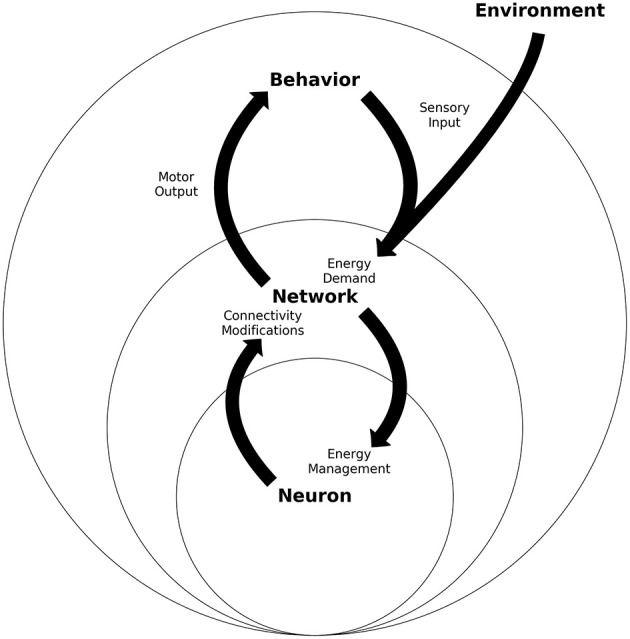
\includegraphics{energy_minimization_local_and_global.jpg}
 \label{fig:2.2}
 \caption{Local energy minimization coellesces in global intelligence. Individual neuronal activation frequency be interpretted as a fast adaptation to energy regulation. On the network scale, this   Explain in detail what's happening in this figure. \dots Intelligent behavior minimizes the energy stress imposed by the organism's sensors and actuators. Reprinted with permission from \cite{Vergara2019}.}
\end{wrapfigure}

The brain exemplifies the principle of free energy minimization. Consuming 20\% of the average human's (CHECK) basal metabolic energy in an organ only 1.5 kg. (3 lbs.) (CHECK), it quickly dies in the abscense of a steady flow of energy. The brain cannot simply maintain large internal energy reserves because the limited signal routing speed of neurons favors maximum packing density. The challange is therefore on individual eurons to remain extremely sensitive to extracellular energy and balance a tight budget. Energetically expensive processes like generating spike trains -- especially over long axons -- must kept to a bare minimum. However energy excess is equally dangerous; unchecked, hyperglyemia leads to neuroinflammation and ultimately, cell death. To cope with energy stress in either direction, neurons regulate nonessential energy consuming or producing processes according to free energy availability. If energy is short, cell synaptic junctions become more resistive and the spiking threshold increases. This decreases the frequency of energetic signaling. Over longer time scales, outgoing dentritic count may even decrease. On the other hand, if there is leftover energy after regular cell processes occur, signal cascades tune the neuron to increase sensitive to its present and potential neuron neighbors: synaptic junctions become less resistive, the spiking thresholds decreases, and cell growth increases -- even branching out to form new dendrites. In either case, the neuron adapts to maintain dynamic equalibrium between energy supply and demand. Of course, essential cell maintenance processes regularize this adaptation to prevent it from collapsing to zero. The network scale effect is: steady free energy minimization contributes positively to information processing. In turn, this local principle promotes global intelligence. (See Figure \ref{fig:2.2}) Experiments have shown that even in the abscence of a reward system or natural body, this local energy stress is a sufficent reward signal for isotropic sections of cortical tissue to learn robotic vehicle control. \cite{Vergara2019}

It comes as no surprise therefore that estimated cost minimization is the norm in behavioral psychology and emergant sciences: humans continually look for ways to increase their efficency or otherwise minimize cognitive and physical workload (MAKE SURE THIS IS A GOOD DEFINITION OF COST ESTIMATION); The global economy likewise . . . These principles extend directly to the research and development of AI. Human cognitive and financial energy form selective pressures to artificial intelligence survival.

This analysis prompts the question:

\begin{center}
Can we make AI systems that autonomously minimize their own energetic demands?
\end{center}

The objective is not only to minimize loss, but every step of optimization: data collection, training ops, compute allocation, and even financial cost minimization. Most AI systems are blind to their own demands: production optimizers recieve little feedback, and few learn to interpret and respond to validation-hyperparameter metrics the way a machine learning engineer does; while roboticists are keenly aware of the tight energy budget, embodied reinforcement learning agents are simultated as if energy is an inexhaustable resource;\footnote{It is beneficial though that purely unsupervised information theoretic objective such as curiosity, empowerment, and skill discovery also converge to energy minimizing behaviors. This is not coincidence though when considering the relationship information theory makes.} data hungry training loops often iterate uniformly over a training distribution when only a few peices of data have information to the model; and it's usually humans rather than AI who bear the cost function when a neural network wants to run another epoch. 

Unlike controlled, artificial intelligence, when wild, natural intelligence demands more energy than expected, it gathers, forages, or hunts independant from humans. This enables the organism to not only collect the nutrients it needs but also do so in an energy efficent manner. The dual energy-efficency, efficent-at-collecting-energy loop of animal life has proved robust over billions of years. It is very intuitive therefore to apply these concepts to a machine learning theory of information metabolism. If data is analogous to food and training, to anabolic processes, then most machine learning pipelines are infants. They are data-hungry and must be spoon-fed. On the other hand, intelligent artificial intelligence is one that learns and autonomously decides when to collect data, what kind of and how much data to collect, and when to start and stop training. Autonomous data \textit{collection} is a leap beyond our ealier thought of autonomous data \text{selection} for it introduces automation to every step of the data collection and preparation pipeline: problem identification, sampling, observation, scraping, or surveying, filtering, cleaning, shifting and scaling, and dataset packaging.

Autonomous data collection and training would not likely collect an uncountable amount of data with respect to the number of tasks it performs. Returning to the free energy principle: excessive energetic intake is just as taxing as unbalanced expendature. Likewise, infants pay greatest attention stimulii that are neither too boring nor suprising. Machine learning recognizes this trend: training on stationary data must often be terminated at a cetain point to prevent overfitting, mode collapse, and simply remain efficent, and the same for non-stationary data may lead to entangled representations or catastrophic forgetting. In deep reinforcement learning, overfitting the training reward function causes decrease in true utility, `cheating' the simulator, and learns dangerous policies. After general pretraining, efficent, autonomous data collection would likely only need well chosen, discrete samples to retain the performance of a few-shot training system just as animals often obtain most environment information when entering a new scene and then operate according to an internal world model only performing visual fixations on objects of uncertainty.\cite{sahni2021hard}

Sampling data before feeding it to the machine learning pipeline has the bonus of adaptive, rather than passive, data poisoning detection. With long-term memory and one shot inference capabilities, detecting one malicious data element would be sufficent to recognize arbitrarily modified pathogens in the future in a way reminiscent of the mammilian immune system.

Natural life intelligently responds to the energy scarcity of every individual day and adjusts its physiological and behavioral characteristics appropriately. This may mean sacrificing exploratory or social behaviors for more immediantly energy-rewarding ones like foraging or hunting. A remarkable adaptation of the brain when insufficently rested or otherwise taxed is that some of its individual neurons decrease their activity or even sacrifice their life to increase the energy availability for the whole. AutoML and neural architecture design already penalize static compute resource use, and sparse mixture of expert models echo similar behaviors by only dynamically routing to a subset of the model for any inference step, however the fully-energy concious AI system has yet to be realized. 
